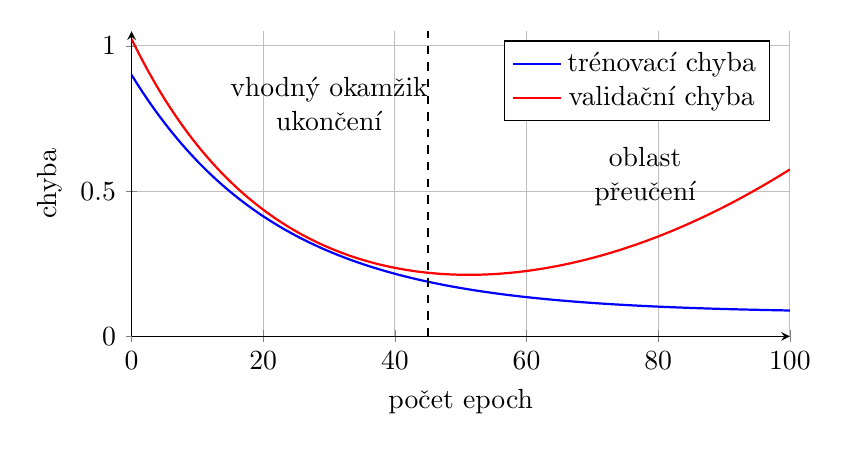
\begin{tikzpicture}
    \begin{axis}[
        width=0.82\textwidth,
        height=0.45\textwidth,
        xmin=0, xmax=100,
        ymin=0, ymax=1.05,
        axis lines=left,
        xlabel={počet epoch},
        ylabel={chyba},
        xlabel near ticks,
        ylabel near ticks,
        legend pos=north east,
        grid=both,
        domain=0:100,
        samples=120
    ]

        \addplot[thick, blue]
            {0.82*exp(-0.045*x)+0.08};
        \addlegendentry{trénovací chyba}

        \addplot[thick, red]
            {0.58*exp(-0.060*x)+0.18+0.00013*(x-45)^2};
        \addlegendentry{validační chyba}

        \draw[dashed, thick]
            (axis cs:45,0) -- (axis cs:45,1.05);

        \node[align=center]
            at (axis cs:30,0.80)
            {vhodný okamžik\\ukončení};

        \node[align=center, text width=28mm]
            at (axis cs:78,0.55)
            {oblast\\přeučení};

    \end{axis}
\end{tikzpicture}
